\documentclass{article}
\usepackage[english]{babel}
\usepackage[a4,top=2cm,bottom=2cm,left=3cm,right=3cm,marginparwidth=1.75cm]{geometry}
\usepackage{amsmath}
\usepackage{graphicx}
\usepackage[colorlinks=true, allcolors=blue]{hyperref}

\title{Project 1: Inference of BK initial condition}
\author{Carlisle Aurabelle Casuga}

\begin{document}
\maketitle

\section{MV}

For the initial run on the MV model with 50 design points, sampled using plain latin hypercube sampling within a wide parameter  space with bounds: $Q_{s0}²$ = [0.001, 2.0] 1/GeV²; $C²$ = [0.1, 100.0], and $\sigma_{0}/2$ = [1.0, 40.0] mb, the following results were obtained: 

\begin{figure}[h]
\centering
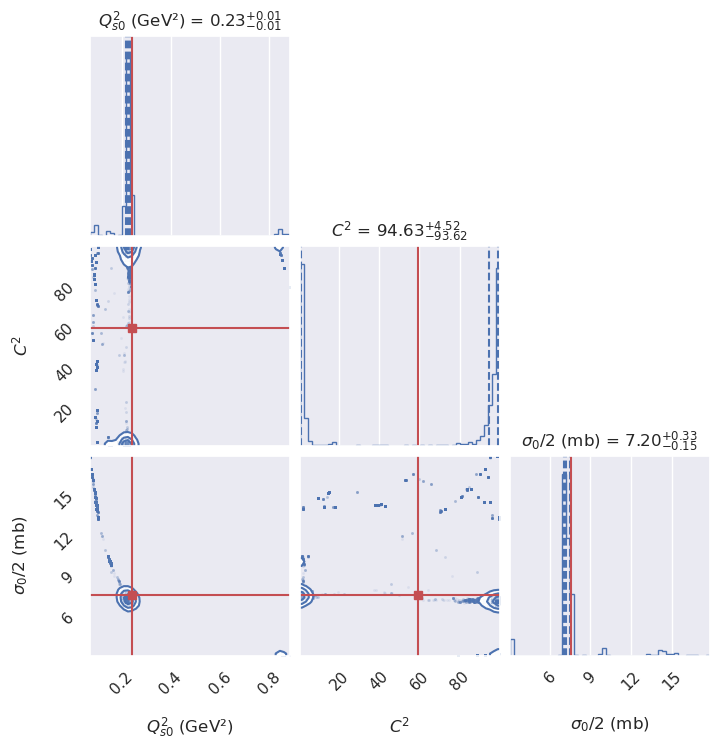
\includegraphics[width=0.5\textwidth]{figs\mv_50d_initial_50w.png}
\caption{Initial run on the MV model with 50 design points}
\label{fig:mv_50d_50w}
\end{figure}

Figure \ref{fig:mv_50_1} is sampled with 50 walkers, total 1500 steps, 500 of which are burn steps. This will provide us with a rough estimate of the posterior distribution of the parameters. Actual values of the parameters at the 16\%, 50\%, and 84\% percentiles are:

$Q_{s0}²$: [(0.16, 0.21728015544863194), (0.5, 0.2275510190337838), (0.84, 0.23450182482460977)]
$C²$: [(0.16, 1.0035763833397198), (0.5, 94.62810202727259), (0.84, 99.14833702805878)]
$\sigma_{0}/2$: [(0.16, 7.052807276014379), (0.5, 7.200058879152208), (0.84, 7.5276927226268135)]

From the 2013 paper, the values of the parameters are: $Q_{s0}²$ = 0.104 GeV²; $C²$ = 14.5, and $\sigma_{0}/2$ = 18.2 mb. We have a large disparity between these values and the values we obtained from the initial run. Next run we can tighten the bounds of $Q_{s0}²$ = [0.001, 0.5] but widen the C² parameters to [0.05, 150.0] to accomodate the peak at large values of C².

We show here the chain of walkers in this run where some of the walkers are stuck in areas of low likelihood. To resolve this, we  double the number of walkers to 100 and run the sampler for 1000 burn steps. Then we (emcee) sample within a tighter space surrounding the posterior distribution peaks. 

\begin{figure}[h]
\centering
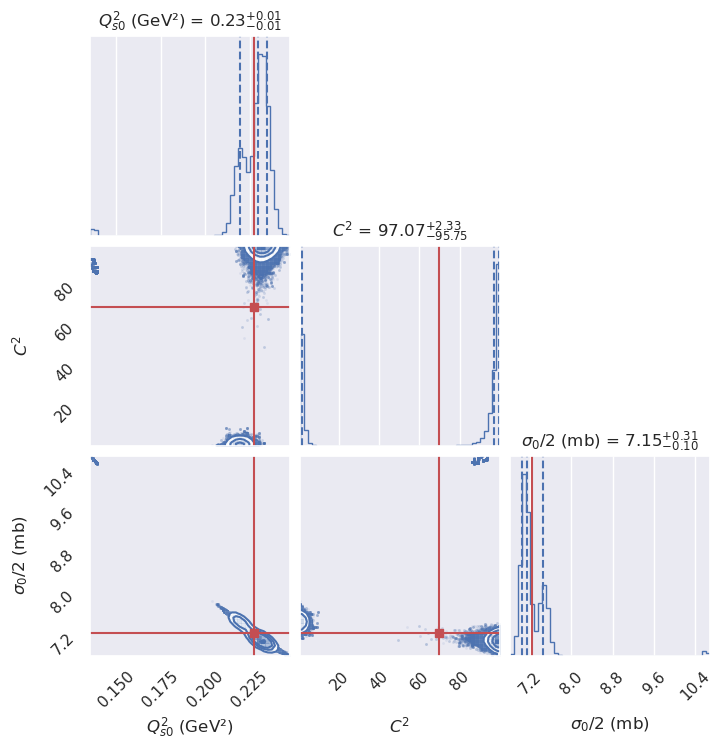
\includegraphics[width=0.5\textwidth]{figs\mv_50d_initial_100w.png}
\caption{Same MV run but with 100 walkers}
\label{fig:mv_50d_100w}
\end{figure}

\section{MVe}

With the MVe model, there are 4 free model parameters to be fitted against: $$Q_{s0}²$$ $$C²$$ $$\sigma_{0}/2$$ with the addition of $$e_c$$. The bounds of the LHS sampling of the parameters are: $Q_{s0}²$ = [0.001, 2.0] 1/GeV²; $C²$ = [0.1, 100.0], and $\sigma_{0}/2$ = [1.0, 40.0] mb. The bounds of $e_c$ are [0.5, 100.0]. In this run we aimed to sample 49 design points through both plain LHS and orthogonal LHS. In both cases the GPE performed very poorly with very large errors and off predictions. The next run is to try with more design points, specifically 121 design points.

The GPE is ran with an RBF + WhiteKernel kernels and whose initial hyperparameters were set at "length_scale = 1 * np.ones(theta.shape[1]), length_scale_bounds = (1e-10, 1e10)" but with the Whitekernel with default parameters. We also set n_restart_optimizer = 2 so that a better fit is made. With these settings there is no error warning regarding the determination of the optimal hyperparameter of the kernels. With 10\% of the training data as validation data and n=5 principal components, the GPE produces the following predictions for a single kinematical point. We also show  the zscore for a single kinematical point.

\begin{figure}[h]
\centering
\includegraphics[width=0.5\textwidth]{figs\mve_121d_gpe.png}
\caption{GPE predictions for a single kinematical point}
\label{fig:mve_121d_gpe}
\end{figure}

\begin{figure}[h]
\centering
\includegraphics[width=0.5\textwidth]{figs\mve_121d_zscore.png}
\caption{Zscore for a single kinematical point}
\label{fig:mve_121d_zscore}
\end{figure}

The emcee sampling for

\end{document}